% TwinArm technical report: the system as built, and its use as a platform for embodied visuomotor studies.
% Build: pdflatex TwinArm_Technical_Report.tex (twice), or latexmk -pdf.
% Data: data/elbow_step.dat (a measured step of the elbow and its fitted model); figures/: interface screenshots.
\documentclass[11pt,a4paper]{article}
\usepackage[T1]{fontenc}
\usepackage[utf8]{inputenc}
\usepackage{lmodern}
\usepackage[margin=2.3cm]{geometry}
\usepackage{amsmath,amssymb}
\usepackage{booktabs,tabularx,array}
\usepackage{siunitx}
\usepackage{xcolor}
\usepackage{graphicx}
\usepackage{tikz}
\usetikzlibrary{arrows.meta,positioning,fit,calc,backgrounds}
\usepackage{pgfplots}
\pgfplotsset{compat=1.18}
\usepackage{caption}
\usepackage{float}
\usepackage{enumitem}
\usepackage[hidelinks]{hyperref}
\usepackage{microtype}

\definecolor{accent}{HTML}{A4161A}
\definecolor{muted}{HTML}{6B6460}
\sisetup{per-mode=symbol,group-separator={\,},range-phrase=--}
\captionsetup{font=small,labelfont=bf}
\setlist{itemsep=2pt,topsep=4pt}
\newcolumntype{L}{>{\raggedright\arraybackslash}X}
\newcommand{\status}[1]{\textsf{\small #1}}
\newcommand{\cmd}[1]{\texttt{#1}}

\title{\textbf{TwinArm}\\[4pt]
\large A wireless leader--follower robotic arm\\ as a platform for embodied visuomotor studies\\[10pt]
\normalsize Technical report}
\date{November 2026}

\begin{document}
\maketitle

\begin{abstract}
\noindent TwinArm is a five-joint robotic arm with a gripper, controlled through a small, passive copy of
itself. The operator moves the leader (master) arm by hand. Contactless magnetic encoders read its joint angles,
and the angles travel over a dedicated radio link or WiFi. A follower arm with high-torque actuators reproduces
the motion joint by joint. The follower can also record a demonstration and replay it on its own.

This report describes the complete system as built: sensing and signal processing on the leader, the
communication link, forward and inverse kinematics, the mapping between the two arms, and the follower's
control. That control is made of the actuators' cascaded PID loops and an outer model predictive controller,
identified from step tests on the real arm. The report also covers the operator application, logging and
commissioning, and gives the measured performance, keeping measured and simulated results apart. A final
section shows how the platform carries a visuomotor adaptation paradigm from a screen task to embodied control
of a robot.
\end{abstract}

\tableofcontents
\bigskip

% ======================================================================================================
\section{Purpose}

Visuomotor adaptation is usually studied with a cursor on a screen: the participant reaches towards targets
while the mapping between hand and cursor is perturbed, for instance rotated by \ang{30}. TwinArm carries this
kind of paradigm to a physical system. The participant steers a real arm by moving a kinematically matched
leader arm, or another input device, and every command, joint angle and event is logged with a timestamp.

The platform brings four properties to such a study:
\begin{itemize}
\item \textbf{Embodied, intuitive control.} The leader is a passive copy of the follower, so a joint of the
      leader turns the same joint of the follower. No abstract mapping has to be learnt before the experiment.
\item \textbf{A fully software-defined mapping.} The mapping from leader to follower runs in one place, so it
      can be perturbed (rotated, offset or delayed) under experimental control.
\item \textbf{Measured, repeatable actuation.} Every joint's response is identified from step tests. The
      follower's static error is a few hundredths of a degree (Section~\ref{sec:results}).
\item \textbf{An operator outside the robot's workspace.} The link is wireless, so the participant works at a
      safe distance from a high-torque arm.
\end{itemize}

% ======================================================================================================
\section{System overview}

Figure~\ref{fig:arch} shows the two arms and the links between them; Table~\ref{tab:hw} lists the hardware.

\begin{figure}[ht]
\centering
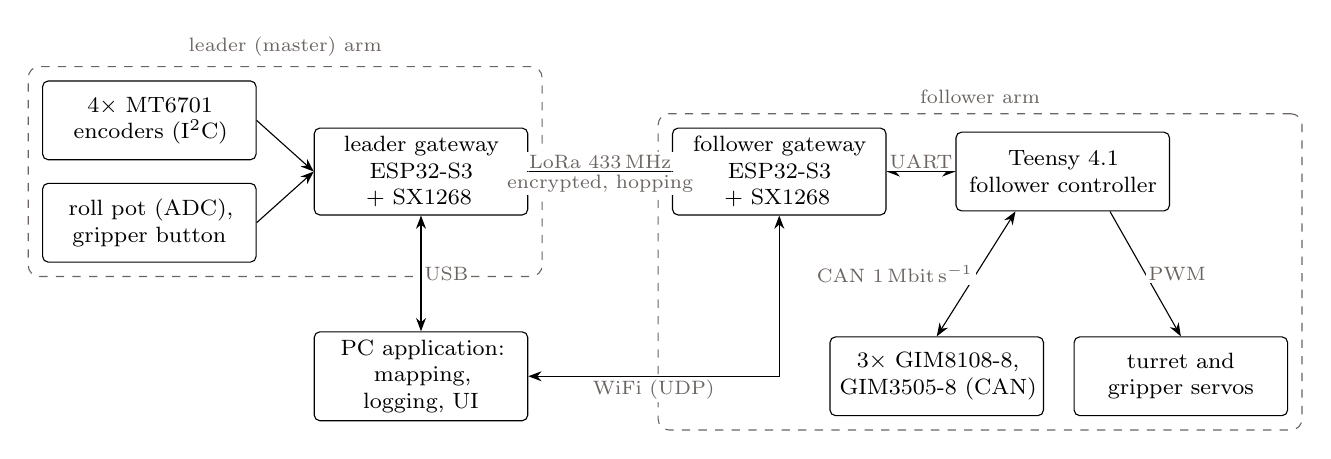
\begin{tikzpicture}[font=\small, >=Stealth,
  box/.style={draw, rounded corners=2pt, align=center, minimum height=10mm, text width=25mm, inner sep=3pt,
              fill=white, font=\footnotesize},
  grp/.style={draw=muted, dashed, rounded corners=4pt, inner sep=5pt},
  lab/.style={font=\scriptsize, text=muted, fill=white, inner sep=1pt}]
  \node[box] (enc) at (0,0.65) {4$\times$ MT6701\\ encoders (I$^2$C)};
  \node[box] (pot) at (0,-0.65) {roll pot (ADC),\\ gripper button};
  \node[box] (mgw) at (3.45,0) {leader gateway\\ ESP32-S3 + SX1268};
  \node[box] (pc)  at (3.45,-2.6) {PC application:\\ mapping, logging, UI};
  \node[box] (fgw) at (8.0,0) {follower gateway\\ ESP32-S3 + SX1268};
  \node[box] (teensy) at (11.6,0) {Teensy 4.1\\ follower controller};
  \node[box] (can) at (10.0,-2.6) {3$\times$ GIM8108-8,\\ GIM3505-8 (CAN)};
  \node[box] (servo) at (13.1,-2.6) {turret and\\ gripper servos};
  \draw[->] (enc.east) -- (mgw.west);
  \draw[->] (pot.east) -- (mgw.west);
  \draw[<->] (mgw) -- node[lab, right] {USB} (pc);
  \draw[<->] (mgw) -- node[lab, above] {LoRa \SI{433}{\mega\hertz}} node[lab, below] {encrypted, hopping} (fgw);
  \draw[<->] (pc.east) -- node[lab, below] {WiFi (UDP)} (8.0,-2.6) -- (fgw.south);
  \draw[<->] (fgw) -- node[lab, above] {UART} (teensy);
  \draw[<->] (teensy.south) ++(-0.6,0) -- node[lab, left] {CAN \SI{1}{\mega\bit\per\second}} (can.north);
  \draw[->] (teensy.south) ++(0.6,0) -- node[lab, right] {PWM} (servo.north);
  \begin{scope}[on background layer]
    \node[grp, fit=(enc)(pot)(mgw), label={[font=\scriptsize, text=muted]above:leader (master) arm}] {};
    \node[grp, fit=(fgw)(teensy)(can)(servo), label={[font=\scriptsize, text=muted]above:follower arm}] {};
  \end{scope}
\end{tikzpicture}
\caption{System architecture. Commands from the PC reach the follower either over WiFi, or over USB to the
leader's gateway and then over the radio. Telemetry returns the same way.}
\label{fig:arch}
\end{figure}

\begin{table}[ht]
\centering\small
\begin{tabularx}{\linewidth}{@{}lL@{}}
\toprule
Part & Role and key figures \\
\midrule
Leader gateway & LightGateway 1.0: ESP32-S3 with an SX1268 LoRa module at \SI{433}{\mega\hertz}; reads the
                 leader arm and is the PC's radio link over USB \\
Leader encoders & 4$\times$ MT6701, \SI{14}{bit} absolute (\ang{0.022}), on a TCA9548A I$^2$C multiplexer:
                 turret, shoulder, elbow, wrist pitch \\
Leader inputs & wrist-roll potentiometer (ADC); a gripper button that toggles open and closed \\
Follower controller & Teensy 4.1 (\SI{600}{\mega\hertz} Cortex-M7, single-precision FPU); microSD for
                 recordings; EEPROM for calibration and joint models \\
Joint actuators & SteadyWin GDZ drivers on one CAN bus: 3$\times$ GIM8108-8 (shoulder, elbow, wrist pitch;
                 rated \SI{7.5}{\newton\metre}, stall \SI{22}{\newton\metre}, datasheet) and a GIM3505-8 (wrist
                 roll, 8:1 gear) \\
Servos & DS5180 turret servo (open loop, 500--\SI{2500}{\micro\second} over \ang{180}); DS3218 gripper
                 (1350--\SI{2000}{\micro\second}) \\
Follower gateway & LightGateway 1.0: WiFi access point (UDP), radio follower, UART to the Teensy \\
Power & actuator bus (22--\SI{24}{\volt}) with a fuse and a hardware emergency stop; separate servo and logic
                 supplies with a common ground \\
\bottomrule
\end{tabularx}
\caption{Hardware.}
\label{tab:hw}
\end{table}

\paragraph{Software.} Four programs make up the system: the leader gateway's firmware, the follower gateway's
firmware, the Teensy's firmware, and a PC application in Python. The two gateways share one radio library. The
Teensy drives the actuators through a header-only CAN driver for the SteadyWin protocol. The PC application
holds the mapping, the user interface, logging and commissioning, together with a simulator of the whole
follower for development without hardware.

% ======================================================================================================
\section{Kinematics}

\subsection{Structure and forward kinematics}

Both arms have the same five joints: a base turret $q_1$ about the vertical axis; shoulder, elbow and wrist
pitch $q_2,q_3,q_4$, with parallel axes, moving the arm in one vertical plane; and the wrist roll $q_5$ about
the tool axis, followed by the gripper. Table~\ref{tab:dh} gives the Denavit--Hartenberg parameters of the
follower. The leader is a geometric copy at \SI{40}{\percent} scale. Uniform scaling leaves the joint angles
unchanged, so the leader's joint angles are the follower's joint commands. The follower reaches
$a_2+a_3+d_5=\SI{0.742}{\metre}$ from its shoulder axis.

\begin{table}[ht]
\centering\small
\begin{tabular}{@{}clcccc@{}}
\toprule
$i$ & joint & $a_i$ (mm) & $\alpha_i$ & $d_i$ (mm) & $\theta_i$ \\
\midrule
1 & turret      & 0   & $\pi/2$ & $d_1$ & $q_1$ \\
2 & shoulder    & 300 & 0       & 0     & $q_2$ \\
3 & elbow       & 300 & 0       & 0     & $q_3$ \\
4 & wrist pitch & 0   & $\pi/2$ & 0     & $q_4+\pi/2$ \\
5 & wrist roll  & 0   & 0       & 142   & $q_5$ \\
\bottomrule
\end{tabular}
\caption{Denavit--Hartenberg parameters of the follower ($d_1$ is the height of the shoulder axis).}
\label{tab:dh}
\end{table}

The tool pose follows from the forward kinematics
\begin{equation}
  \mathbf T_0^5(\mathbf q)=\prod_{i=1}^{5}\mathbf A_i(q_i),\qquad
  \mathbf A_i=\begin{bmatrix}
    c_{\theta_i} & -s_{\theta_i}c_{\alpha_i} & s_{\theta_i}s_{\alpha_i} & a_i c_{\theta_i}\\
    s_{\theta_i} & c_{\theta_i}c_{\alpha_i} & -c_{\theta_i}s_{\alpha_i} & a_i s_{\theta_i}\\
    0 & s_{\alpha_i} & c_{\alpha_i} & d_i\\
    0&0&0&1\end{bmatrix}.
\end{equation}
Because the pitch joints are parallel, the application works with the planar form of the chain. Let $g_1$ be
the upper arm's angle from the horizontal and $g_2,g_3$ each angle relative to the previous link, with
absolute angles $\phi_k=\sum_{j\le k}g_j$ and $(l_1,l_2,l_3)=(300,300,142)$~mm. The tool tip in the arm's plane
and the tool angle are
\begin{equation}
  \mathbf p=\begin{bmatrix}p_x\\ p_y\end{bmatrix}=\sum_{k=1}^{3} l_k\begin{bmatrix}\cos\phi_k\\ \sin\phi_k\end{bmatrix},
  \qquad \psi=\phi_3 .
\end{equation}
The turret turns this plane about the vertical axis, so in a frame with $X$ forward, $Y$ to the left and $Z$ up
the tip is at
\begin{equation}
  \mathbf P=\bigl(p_x\cos q_1,\; p_x\sin q_1,\; d_1+p_y\bigr).
\end{equation}
Each joint's angle from the arm's zero pose maps to the drawn angle as $g_k=g_k^{0}+\sigma_k q_k$, with the
drawn angle $g_k^0$ of the zero pose and the motor's direction $\sigma_k=\pm1$.

\subsection{Inverse kinematics}

When the tool tip is dragged in the application, the pitch joints are found for a target tip $\mathbf p^*$ and
a tool angle $\psi^*$ held from the moment the drag starts. The wrist point is
\begin{equation}
  \mathbf w=\mathbf p^*-l_3\begin{bmatrix}\cos\psi^*\\ \sin\psi^*\end{bmatrix},\qquad r=\lVert\mathbf w\rVert .
\end{equation}
If $|l_1-l_2|\le r\le l_1+l_2$, the two-link chain has the closed-form solutions
\begin{gather}
  g_2=\pm\arccos\frac{r^2-l_1^2-l_2^2}{2l_1l_2},\\
  g_1=\operatorname{atan2}(w_y,w_x)-\operatorname{atan2}\!\bigl(l_2\sin g_2,\;l_1+l_2\cos g_2\bigr),\qquad
  g_3=\psi^*-g_1-g_2 ,
\end{gather}
one per elbow branch. Each solution is first brought into its joint's range. A solution is accepted only if it
is inside every joint limit and no joint moves more than \ang{30} from the current pose. A larger jump would be
a flip to the other branch, not a step. Of the solutions that pass, the one closest to the current pose is
taken.

When the target is out of reach, past a limit, or would need a branch flip, damped least squares (DLS) walks
from the current pose to the closest pose it can reach. The task is the tip position and the tool angle, the
angle weighted by $w_\psi=0.3\,l_3$ (millimetres per radian), so that the tool angle gives way first:
\begin{equation}
  \mathbf e=\begin{bmatrix}\mathbf p^*-\mathbf p\\ w_\psi(\psi^*-\psi)\end{bmatrix},\qquad
  J=\begin{bmatrix}
    -p_y & -(l_2 s_{\phi_2}+l_3 s_{\phi_3}) & -l_3 s_{\phi_3}\\
    p_x & l_2 c_{\phi_2}+l_3 c_{\phi_3} & l_3 c_{\phi_3}\\
    w_\psi & w_\psi & w_\psi \end{bmatrix},
\end{equation}
\begin{equation}
  \Delta\mathbf g=J^{\mathsf T}\bigl(JJ^{\mathsf T}+\mu^2 I\bigr)^{-1}\mathbf e,\qquad \mu=20 .
\end{equation}
Each step is scaled so that no joint moves more than \SI{0.1}{\radian} (which keeps the walk on one branch),
then clamped to the joint limits. The iteration stops when $\lVert\mathbf e\rVert_\infty<0.05$ or after 200
steps. Finally the elbow, the wrist and the tip must stay at least \SI{15}{\milli\metre} above the table;
otherwise the arm keeps its previous pose.

% ======================================================================================================
\section{Sensing and signal processing on the leader}

\paragraph{Joint encoders.} The four MT6701 sensors are read over I$^2$C at \SI{400}{\kilo\hertz} through the
multiplexer. A reading takes both angle bytes in one transfer, so the two halves of the \SI{14}{bit} value
always come from the same sample: $\theta=\frac{360}{16384}\,(b_{\mathrm{hi}}\cdot 2^6+\lfloor b_{\mathrm{lo}}/4\rfloor)$.
A sensor that does not answer is reported as \emph{no reading}, never as an angle.

\paragraph{Wrist-roll potentiometer.} The wiper is sampled about once a millisecond. Each frame sends the mean of
the samples of the last \SI{40}{\milli\second}:
\begin{equation}
  \bar v=\frac1K\sum_{t_i>t-\SI{40}{\milli\second}} v_i .
\end{equation}
The window is two whole periods of the \SI{50}{\hertz} mains, so pickup from the mains cancels. When the samples
of the window spread over more than \SI{12}{\percent} of the travel ($\max v_i-\min v_i>490$ counts), the frame
is sent as \emph{no reading}: that spread is the signature of a wiper off its track. On the PC, the readings
$p_k$ (in percent) go through a three-sample median, a low-pass and a hysteresis:
\begin{gather}
  \tilde p_k=\operatorname{median}(p_{k-2},p_{k-1},p_k),\qquad
  f_k=f_{k-1}+\alpha\,(\tilde p_k-f_{k-1}),\quad \alpha=0.25,\\
  h_k=\begin{cases}f_k-b & f_k>h_{k-1}+b\\ f_k+b & f_k<h_{k-1}-b\\ h_{k-1}&\text{otherwise}\end{cases},
  \qquad b=\SI{0.6}{\percent}.
\end{gather}
After the wiring was repaired, the frame-to-frame jitter of the potentiometer is \SI{0.12}{\percent} of its
travel (standard deviation), about \ang{0.3} of wrist roll.

\paragraph{Gripper button.} The button is debounced (\SI{30}{\milli\second}) and toggles the gripper between
open and a configurable closed position. The closed position is configurable so that the digital servo is not
left stalled at full force on an object.

The leader sends its state 20 times a second, over USB to the PC and, over the radio, to the follower.

% ======================================================================================================
\section{Communication}
\label{sec:comm}

\paragraph{Line protocol.} The PC and the follower exchange plain text lines (Appendix~\ref{app:protocol}).
Commands to the follower's console, such as \cmd{2 a12.50} (joint 2 to \ang{12.5} from its zero), go one way;
telemetry comes back. The gateways pass the lines on unchanged. Every \SI{100}{\milli\second} the follower
reports, for each joint, its angle, target, phase current, temperature, bus voltage and current, mode, fault
bits and jam state. It also reports the recorder's state and answers gain reads and step tests on the same
stream.

\paragraph{WiFi.} The follower's gateway opens its own access point. Commands arrive as UDP datagrams and go to
the Teensy over UART at \SI{115200}{baud}; each line from the Teensy returns as one datagram.

\paragraph{Radio.} For untethered use, the two gateways form a dedicated LoRa link at \SI{433}{\mega\hertz}
(spreading factor 5, \SI{500}{\kilo\hertz} bandwidth, coding rate 4/5, \SI{10}{dBm}). The leader paces it in
time slots
\begin{equation}
  T_{\mathrm{slot}}=T_{\mathrm{air}}(\text{leader frame})+T_{\mathrm{air}}(\text{follower frame})
    +\SI{3}{\milli\second}+\SI{6}{\milli\second}\approx\SI{35}{\milli\second}
\end{equation}
(reply delay and margin). In each slot the leader sends one frame and the follower answers on the same channel.
The slots hop over 7 channels between 433.3 and \SI{434.5}{\mega\hertz}. Every block of 7 slots uses each
channel once, in an order shuffled from the session key.

\paragraph{Security.} Both gateways hold the same 128-bit pre-shared key $K$, which never goes on air. A
connection starts with a challenge--response. The leader sends a random nonce $n_M$, and the follower answers
with its own nonce $n_F$ and a proof $\mathrm{HMAC}_K(\texttt{F}\Vert n_M\Vert n_F)$; the leader confirms with
$\mathrm{HMAC}_K(\texttt{M}\Vert n_M\Vert n_F)$. Both ends then derive
\begin{equation}
  S=\mathrm{HMAC\text{-}SHA256}_K(\texttt{K}\Vert n_M\Vert n_F),
\end{equation}
whose first 16 bytes are the session's AES-128 key and whose next 4 bytes seed the hopping order. Every frame
is encrypted and authenticated with AES-128-GCM under the session key, with an 8-byte tag. Its type and slot
number are sent in the clear but authenticated, and the slot number is the nonce. A forged frame fails the tag,
and a replayed one fails the slot check. The payload carries the leader's state (11 bytes: four joints, the
potentiometer and the gripper) and a chunk of the line stream. A chunk that is not acknowledged is sent again
in the next slot, on another channel. If no valid frame arrives for \SI{500}{\milli\second}, both ends return
to the handshake.

\begin{table}[ht]
\centering\small
\begin{tabularx}{\linewidth}{@{}lLl@{}}
\toprule
Quantity & Value & Basis \\
\midrule
Leader state rate & \SI{20}{\hertz} & design \\
Follower telemetry rate & \SI{10}{\hertz} per joint & design \\
Command rate from the application & \SI{20}{\hertz}: changed values, and all of them every \SI{0.5}{\second}
  & design \\
Step-test sampling & \SI{100}{\hertz} & design \\
Radio slots & 28--29 per second & measured \\
Radio frames delivered & 96--\SI{100}{\percent} & measured \\
Round trip over the radio & 63--\SI{78}{\milli\second} idle; about \SI{115}{\milli\second} with full telemetry
  & measured \\
\bottomrule
\end{tabularx}
\caption{Rates and timing.}
\label{tab:timing}
\end{table}

% ======================================================================================================
\section{Mapping from leader to follower}

The mapping runs in the PC application at \SI{20}{\hertz}. For the turret, shoulder, elbow and wrist pitch,
the follower's angle from its zero pose is the leader encoder's turn from a captured reference pose:
\begin{equation}
  q_{f,j}=d_j\,\operatorname{wrap}\!\left(\theta_{m,j}-\theta_{m,j}^{0}\right),\qquad
  \operatorname{wrap}(x)\in[-\ang{180},\ang{180}).
\end{equation}
Here $\theta_{m,j}^{0}$ is the leader's reading when it is held in the follower's zero pose, captured with one
command, and $d_j=\pm1$ sets the direction. The wrist roll follows the filtered potentiometer reading $h$:
\begin{equation}
  q_{f,5}=s\,(h-p_0)\,\frac{T}{100}-\varphi,
\end{equation}
with the potentiometer's zero $p_0$, its travel $T$ in degrees of roll (measured with a two-point calibration),
its direction $s$, and an offset $\varphi=\ang{90}$ that puts the follower's neutral roll near the middle of the
potentiometer. The gripper follows the button. Every command is limited to the joint ranges and checked against
the table with the forward kinematics. A value is sent when it changes by more than \ang{0.05}, and every value
is sent again each \SI{0.5}{\second}.

\paragraph{Pick-up interlock.} When control starts, the leader is rarely in the follower's pose. Each joint
therefore holds until the leader comes to it. Let $\delta_k=q_{f}^{*}-q_{f}$ be the gap between what the leader
asks of a joint and where the follower holds it. The joint picks up when
\begin{equation}
  |\delta_k|\le\ang{5}\quad\text{or}\quad\operatorname{sign}\delta_k\ne\operatorname{sign}\delta_{k-1}
  \;\text{with}\;|\delta_k-\delta_{k-1}|<\ang{90},
\end{equation}
that is, when the leader comes within the window or goes past the joint between two frames. From then on the
joint copies the leader. A wrong reference pose or a reversed direction shows up as a joint that never picks up,
rather than one that swings away.

% ======================================================================================================
\section{Follower control}
\label{sec:control}

\subsection{Inner loops, start-up and supervision}

Each SteadyWin driver closes its own cascaded loops: position, then velocity, then current with field-oriented
control, at about \SI{1}{\kilo\hertz} according to the manufacturer. The Teensy sends position set-points over
CAN, each a request answered by the driver. The drivers restart their multi-turn count at power-up, so every
start homes the joints. All joints home at the same time, at \SI{10}{rpm}, to their drivers' origin, and the
gripper opens and closes once meanwhile. When every joint has settled (under \ang{0.1} in
\SI{200}{\milli\second}), each moves on by a calibrated offset to the arm's zero pose. The offsets can be set in
place: with the arm in the desired pose, one command stores each joint's offset in EEPROM.

\paragraph{Jam detection.} Each \SI{100}{\milli\second}, a joint in position mode counts as stuck if
\begin{equation}
  |q^*-q|>e_j\quad\text{and}\quad|\Delta q|<\min\!\left(\tfrac14\,\omega_{\lim}\,T,\;\ang{1}\right),
\end{equation}
with the tolerance $e_j=\ang{4}$, the joint's speed limit $\omega_{\lim}$ and the period $T$. A joint stuck for
\SI{400}{\milli\second} is jammed: it holds where it stopped and refuses further moves until it is cleared.

\subsection{Identified joint models}

A step test moves one joint by $\pm$\ang{5} from where it is and samples it every \SI{10}{\milli\second} for
\SI{2}{\second}. With the normalised response $\rho(t)=(y(t)-y_0)/\Delta$, the application computes:
\begin{itemize}
\item the overshoot $M_p=\max_t\rho-1$ and the rise time between \SI{10}{\percent} and \SI{90}{\percent};
\item the settling time, the last exit from the band $\max(0.05,\,\ang{0.2}/|\Delta|)$ around 1;
\item the steady-state error $|1-\bar\rho|\,|\Delta|$, with $\bar\rho$ the mean over the last
      \SI{20}{\percent} of the capture;
\item the peak speed, from differences over three samples, compared with the speed limit sent to the driver.
\end{itemize}
Seen from the Teensy, each joint with its inner loops behaves as a second-order system,
\begin{equation}
  \ddot y=\omega_n^2\,(u-y)-2\zeta\omega_n\,\dot y,\qquad |\dot y|\le v_{\max},
  \label{eq:model}
\end{equation}
where $u$ is the position set-point and $y$ the joint angle. The parameters minimise the squared error between
the simulated and the measured curve: a coarse grid over $\omega_n$ and $\zeta$ (with and without a speed cap),
refined by a local search with shrinking multiplicative steps. A cap is kept only when it explains clearly more
of the curve than measurement noise. Table~\ref{tab:models} and Figure~\ref{fig:step} show the result.

\begin{table}[ht]
\centering\small
\begin{tabular}{@{}lccccc@{}}
\toprule
Joint & $\omega_n$ (rad/s) & $\zeta$ & overshoot & settling time & steady-state error \\
\midrule
Shoulder    & 12.0 & 0.37 & \SI{31}{\percent}  & \SI{0.92}{\second} & \ang{0.054} \\
Elbow       & 14.9 & 0.52 & \SI{13}{\percent}  & \SI{0.33}{\second} & \ang{0.014} \\
Wrist pitch & 39.7 & 1.96 & \SI{0.9}{\percent} & \SI{0.34}{\second} & \ang{0.030} \\
Wrist roll  & 68.9 & 2.98 & \SI{0.8}{\percent} & \SI{0.27}{\second} & \ang{0.017} \\
\bottomrule
\end{tabular}
\caption{Joint models and step responses measured on the real arm ($\pm$\ang{5} steps, mean of both
directions). The shoulder's driver gains have been retuned since this test to reduce its overshoot.}
\label{tab:models}
\end{table}

\begin{figure}[ht]
\centering
\begin{tikzpicture}
\begin{axis}[width=0.62\linewidth, height=5.2cm, xlabel={time (s)}, ylabel={elbow angle (\si{\degree})},
  xmin=0, xmax=2, ymin=-0.5, ymax=6, grid=major, grid style={gray!20}, legend pos=south east,
  legend style={font=\small, draw=none}, tick label style={font=\small}, label style={font=\small}]
  \addplot[very thick, black] table[x=t, y=meas] {data/elbow_step.dat};
  \addlegendentry{measured on the arm}
  \addplot[thick, accent, dashed] table[x=t, y=model] {data/elbow_step.dat};
  \addlegendentry{identified model}
\end{axis}
\end{tikzpicture}
\caption{A \ang{5} step of the elbow, measured at \SI{100}{\hertz}, and the fitted model
($\omega_n=\SI{13.1}{\radian\per\second}$, $\zeta=0.64$); the model is within \ang{0.10} RMS of the
measurement.}
\label{fig:step}
\end{figure}

\paragraph{Tuning.} From the metrics, the application suggests changes to the driver's position and velocity
gains. Table~\ref{tab:tune} lists the rules; each round is applied, measured again and repeated.

\begin{table}[ht]
\centering\small
\begin{tabularx}{\linewidth}{@{}lL@{}}
\toprule
Observation & Suggestion \\
\midrule
overshoot above \SI{25}{\percent}, or ringing & position $K_p\times0.8$, velocity $K_p\times1.3$ \\
overshoot of 10--\SI{25}{\percent} & velocity $K_p\times1.2$ (more damping) \\
slow, clean rise (over \SI{0.4}{\second}, under \SI{2}{\percent} overshoot) & position $K_p\times1.25$ \\
steady error above $\max(\ang{0.3},\,0.03|\Delta|)$ & velocity $K_i\times1.5$ \\
rise limited by the speed limit, or a steady cruise far below it & no gain change: the limit, not the loop,
  sets the speed \\
\bottomrule
\end{tabularx}
\caption{Tuning rules applied to each step response.}
\label{tab:tune}
\end{table}

\subsection{Model predictive control over the inner loops}

An outer model predictive controller (MPC) runs on the Teensy every $\Delta t=\SI{20}{\milli\second}$, above
the drivers' loops (Figure~\ref{fig:loop}). The model~\eqref{eq:model} is discretised by integrating one tick
in 20 substeps $h=\Delta t/20$ of semi-implicit Euler,
\begin{equation}
  \dot y\leftarrow\dot y+h\bigl(\omega_n^2(u-y)-2\zeta\omega_n\dot y\bigr),\qquad y\leftarrow y+h\,\dot y ,
\end{equation}
which gives $x_{k+1}=Ax_k+Bu_k$ with $x=[y\;\dot y]^{\mathsf T}$. Over a horizon of $N=25$ ticks
(\SI{0.5}{\second}), the predicted angles are $\hat{\mathbf y}=S_xx_k+S_u\mathbf u$, with the rows of $S_x$ equal
to $CA^{i}$ and $S_u$ lower triangular with entries $CA^{i-j}B$. The controller solves
\begin{equation}
\begin{aligned}
  \min_{\mathbf u}\;& \bigl\lVert S_xx_k+S_u\mathbf u-\mathbf r\bigr\rVert^2+\lambda\bigl\lVert D\mathbf u-\mathbf d\bigr\rVert^2\\
  \text{s.t.}\;& r_{k+i+1}-\ang{25}\le u_{k+i}\le r_{k+i+1}+\ang{25},\qquad i=0,\dots,N-1,
\end{aligned}
\end{equation}
where $D$ takes first differences, $\mathbf d=[u_{k-1},0,\dots,0]^{\mathsf T}$ and $\lambda=0.05$. This is a
quadratic programme with Hessian $H=S_u^{\mathsf T}S_u+\lambda D^{\mathsf T}D$ and linear term
$\mathbf g=S_u^{\mathsf T}(S_xx_k-\mathbf r)-\lambda D^{\mathsf T}\mathbf d$. Its constraints are a box, so the
projection onto them is a clamp, and FISTA (accelerated projected gradient) solves it:
\begin{equation}
\begin{aligned}
  \mathbf u^{(j+1)}&=\Pi_{\mathrm{box}}\!\left(\mathbf z^{(j)}-\tfrac1L\bigl(H\mathbf z^{(j)}+\mathbf g\bigr)\right),\qquad
  t_{j+1}=\tfrac12\Bigl(1+\sqrt{1+4t_j^2}\Bigr),\\
  \mathbf z^{(j+1)}&=\mathbf u^{(j+1)}+\frac{t_j-1}{t_{j+1}}\bigl(\mathbf u^{(j+1)}-\mathbf u^{(j)}\bigr),
\end{aligned}
\end{equation}
with the step $1/L$ from the largest eigenvalue of $H$ (power iteration, computed once per model). The solver
runs 40 iterations, warm-started from the previous solution shifted by one tick; only $u_k$ is sent. With the
models of Table~\ref{tab:models}, $H$ is well conditioned (condition number 12--86), so 40 iterations converge.
The box keeps every set-point within \ang{25} of what a plain replay would send. An observer estimates angle and
speed from the angle measured over CAN:
\begin{equation}
  \hat x^-=A\hat x+Bu_{k-1},\qquad \hat x=\hat x^-+\begin{bmatrix}0.6\\ 0.3/\Delta t\end{bmatrix}\bigl(y_k-\hat y^-\bigr).
\end{equation}
A solve takes \SI{0.37}{\milli\second} per joint on the Teensy (measured), so the four joints use about
\SI{7}{\percent} of a tick. The joint models are stored in EEPROM and refreshed from every whole-arm test.

\begin{figure}[ht]
\centering
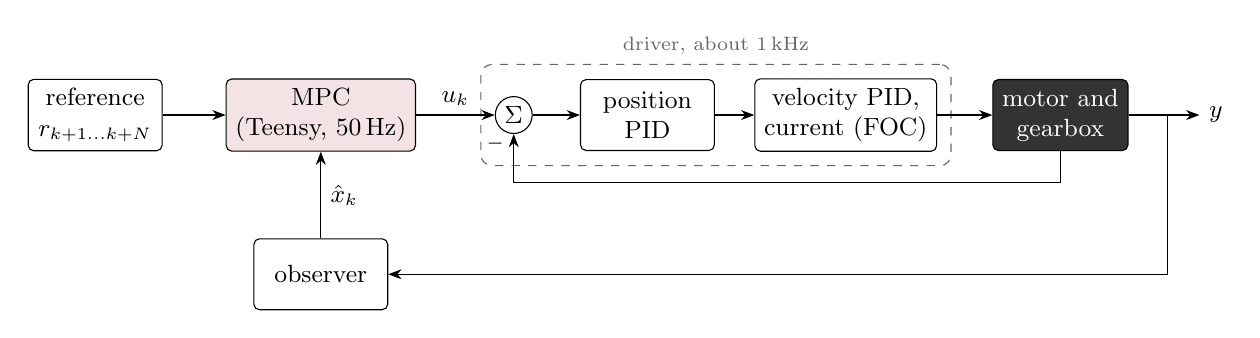
\begin{tikzpicture}[font=\small, >=Stealth,
  blk/.style={draw, rounded corners=2pt, minimum height=9mm, minimum width=17mm, align=center, fill=white},
  sum/.style={draw, circle, inner sep=1.5pt}]
  \node[blk] (ref) {reference\\ $r_{k+1\dots k+N}$};
  \node[blk, right=8mm of ref, fill=accent!12] (mpc) {MPC\\ (Teensy, \SI{50}{\hertz})};
  \node[sum, right=10mm of mpc] (s) {$\Sigma$};
  \node[blk, right=6mm of s] (pp) {position\\ PID};
  \node[blk, right=5mm of pp] (vp) {velocity PID,\\ current (FOC)};
  \node[blk, right=7mm of vp, fill=black!80, text=white] (pl) {motor and\\ gearbox};
  \node[blk, below=11mm of mpc] (obs) {observer};
  \draw[->] (ref) -- (mpc);
  \draw[->] (mpc) -- node[above] {$u_k$} (s);
  \draw[->] (s) -- (pp);
  \draw[->] (pp) -- (vp);
  \draw[->] (vp) -- (pl);
  \draw[->] (pl.east) -- ++(9mm,0) node[right] {$y$};
  \draw[->] ($(pl.south)$) -- ++(0,-4mm) -| node[pos=0.9, left, font=\scriptsize] {$-$} (s.south);
  \draw[->] ($(pl.east)+(5mm,0)$) |- (obs.east);
  \draw[->] (obs) -- node[right] {$\hat x_k$} (mpc);
  \begin{scope}[on background layer]
    \node[draw=muted, dashed, rounded corners=4pt, fit=(s)(pp)(vp), inner sep=5pt,
          label={[font=\scriptsize, text=muted]above:driver, about \SI{1}{\kilo\hertz}}] {};
  \end{scope}
\end{tikzpicture}
\caption{Control structure: the drivers keep their cascaded PID loops; the MPC on the Teensy chooses their
set-points from the identified model and the measured angle.}
\label{fig:loop}
\end{figure}

The MPC acts where the reference is known ahead, that is, on replays.

\subsection{Recording and replay}

While the operator drives the follower, the Teensy can record what it is told: the four joints, the turret and
the gripper, every $T_s=\SI{10}{\milli\second}$, for up to five minutes (stored as hundredths of a degree in
RAM, then saved on the microSD card). A replay runs at a speed factor $\gamma\in[0.1,2]$. It first moves to the
recording's first pose in $T=\operatorname{clamp}\bigl(\max_j|\Delta q_j|/(\SI{20}{\degree\per\second}),\,1,\,8\bigr)$
seconds with a minimum-jerk profile,
\begin{equation}
  q(t)=q_0+\Delta q\,\bigl(10\tau^3-15\tau^4+6\tau^5\bigr),\qquad \tau=t/T .
\end{equation}
It then plays the recording at the index $s(t)=\gamma t/T_s$, read from the clock so that a slow loop does not
stretch the take, through a centred moving average:
\begin{equation}
  \bar q(s)=\frac1{11}\sum_{j=-5}^{5}q\bigl[\lfloor s\rfloor+j\bigr],
\end{equation}
interpolated between samples, sent every \SI{20}{\milli\second} through the MPC. A manual command or a jam stops
it. A replay runs on the Teensy alone, without the PC or the link.

% ======================================================================================================
\section{Operator application}
\label{sec:app}

The PC application connects either over WiFi (an IP address) or, through the leader's gateway, over the radio
(a serial port). Its tabs are \emph{Manual} (control and telemetry), \emph{Configuration} (gains, step tests,
jam detection, joint zeros), \emph{Teach \& Replay} and \emph{Master} (the leader arm, its calibration and the
radio).

\begin{figure}[ht]
\centering
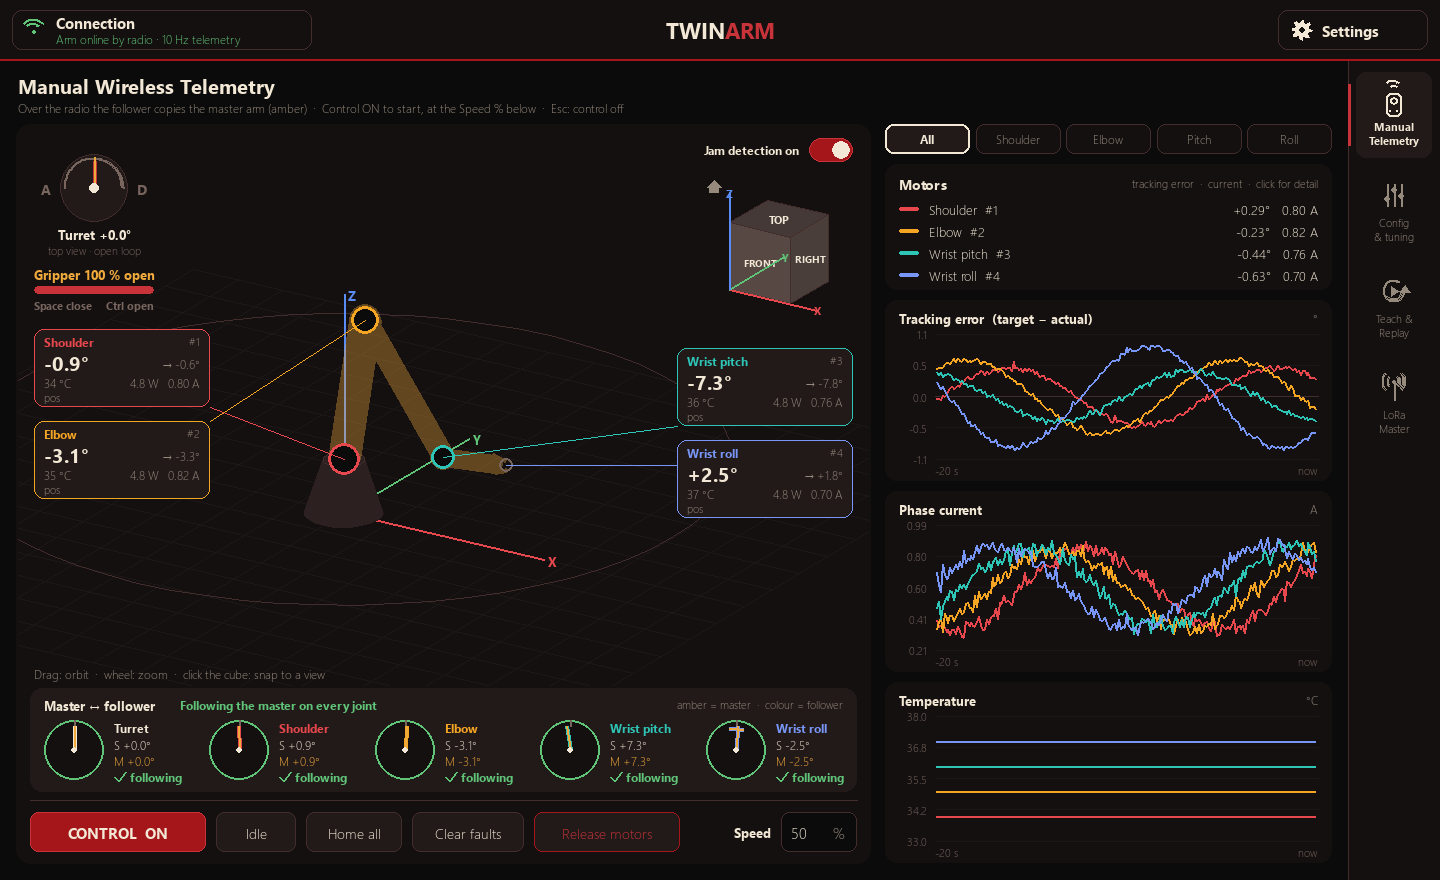
\includegraphics[width=\linewidth]{figures/ui_teleop_3d.png}
\caption{Teleoperation through the leader arm over the radio (the interface with illustrative telemetry). Left:
the follower in 3D on the table grid, with the $X$, $Y$, $Z$ axes, the leader's pose overlaid in amber, and an
orientation cube (click a face to snap the view). Bottom: one dial per joint with the follower (colour) and the
leader (amber), and its pick-up state. Right: tracking error, phase current and temperature of every joint.}
\label{fig:ui3d}
\end{figure}

\paragraph{Teleoperation through the leader.} Over the radio, the follower copies the leader whenever control is
on (Figure~\ref{fig:ui3d}). The 3D view orbits with the mouse; a click on the orientation cube snaps it to the
front, side or top view. Under the view, the alignment strip shows, per joint, the follower's and the leader's
angle on one dial, the gap between them, and whether the joint is lined up, following, or still waiting for the
pick-up. Before control is switched on, it shows whether starting would be smooth.

\begin{figure}[ht]
\centering
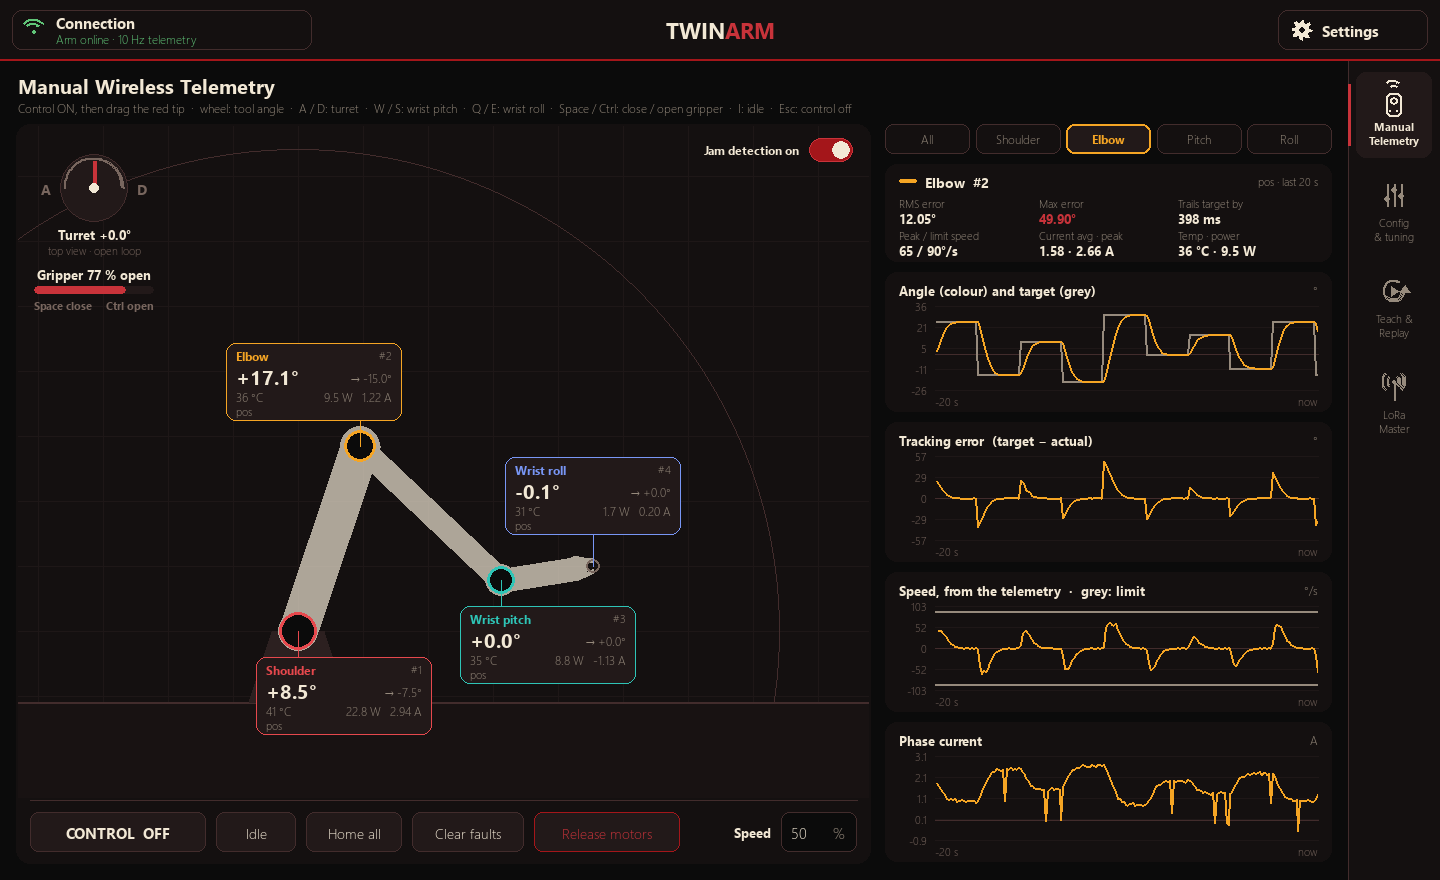
\includegraphics[width=\linewidth]{figures/ui_scope_wifi.png}
\caption{Direct control over WiFi (the simulator). Left: the side view, where the tool tip is dragged with the
inverse kinematics. Right: one joint as a control loop: angle and target, tracking error, speed against its
limit, phase current, with the RMS and maximum error, the lag behind the target, peak speed against the limit,
current, temperature and power.}
\label{fig:uiscope}
\end{figure}

\paragraph{Direct control.} Over WiFi the operator can also drive the follower without the leader
(Figure~\ref{fig:uiscope}). Dragging the red tool tip moves the arm through the inverse kinematics, and the
mouse wheel turns the tool angle. Keys turn the turret, tilt the wrist, roll it and close the gripper, each at
its joint's speed limit, so the target never runs ahead of the motor. A per-joint panel shows the joint as a
control loop. The lag behind the target is estimated as the shift $\tau$ that best aligns the measured angle
with the target,
\begin{equation}
  k^*=\arg\min_{0\le k\le 15}\;\frac1{n-k}\sum_{i=1}^{n-k}\bigl(y_{i+k}-r_i\bigr)^2,\qquad
  \tau=k^*\,\overline{\Delta t},
\end{equation}
over the samples $y_i$, $r_i$ of the plotted window, with $\overline{\Delta t}$ their mean spacing; $k^*$ is
refined between samples by a parabola through the costs around the minimum.

\begin{figure}[ht]
\centering
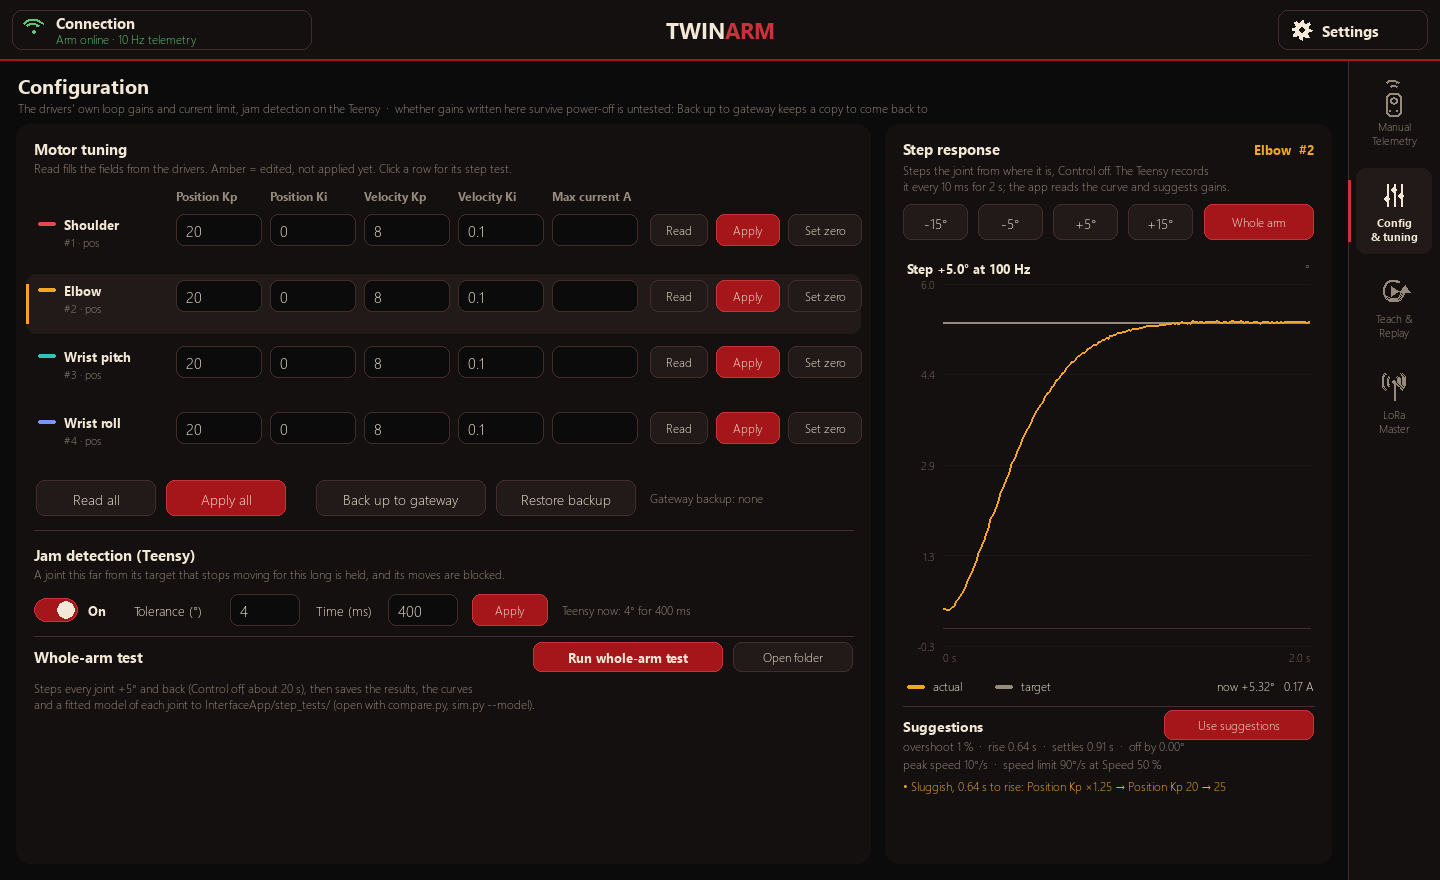
\includegraphics[width=\linewidth]{figures/ui_config_step.png}
\caption{Commissioning (the simulator): the drivers' gains per joint, a step response sampled at
\SI{100}{\hertz} with its metrics, and the suggested gain changes.}
\label{fig:uiconfig}
\end{figure}

\paragraph{Commissioning.} The Configuration tab (Figure~\ref{fig:uiconfig}) reads and writes the drivers'
position and velocity gains and current limits, and keeps a backup of the gains in the follower gateway's
flash. It runs the step tests with their metrics and gain suggestions. It also runs a whole-arm test, which steps
every joint by $+\ang{5}$ and $-\ang{5}$, writes the results and curves to CSV and fits the joint models, which
the application then sends to the Teensy's MPC. It sets the jam detection, and stores a joint's zero where it
stands.

\paragraph{Logging.} Every session is logged automatically: each line sent or received, which includes the
leader's state, the follower's telemetry and every command, with a timestamp relative to the start of the
connection. Step tests are kept as CSV files with their fitted models. An unattended test script runs holds,
steps and gain sets over WiFi with safety limits and logs all of them for later analysis.

% ======================================================================================================
\section{Safety}

The follower is a high-torque arm, so the system keeps the operator out of its workspace and bounds its motion
in several layers:
\begin{itemize}
\item a hardware emergency stop on the actuator bus;
\item joint and turret limits, a speed limit on every joint, and a table check on every command;
\item the pick-up interlock, so that nothing jumps when control starts;
\item jam detection, which holds a joint that stalls short of its target;
\item a link watchdog: without telemetry for a second, control switches off and the arm holds its last pose;
      over the radio, \SI{500}{\milli\second} without a valid frame drops the link;
\item a two-step confirmation for releasing the motors, setting a zero or capturing a reference pose.
\end{itemize}

% ======================================================================================================
\section{Measured performance}
\label{sec:results}

\begin{table}[ht]
\centering\small
\begin{tabularx}{\linewidth}{@{}Lrl@{}}
\toprule
Quantity & Value & Basis \\
\midrule
Leader encoder resolution & \ang{0.022} & \status{design (14-bit)} \\
Follower steady-state error after a step & \ang{0.014}--\ang{0.054} & \status{measured} \\
Model fit to the measured steps (RMS) & \ang{0.06}--\ang{0.17} & \status{measured} \\
Wrist-roll input jitter (after repair) & about \ang{0.3} & \status{measured} \\
Radio slots, frames delivered & 28--29 /s, 96--\SI{100}{\percent} & \status{measured} \\
Radio round trip & 63--\SI{115}{\milli\second} & \status{measured} \\
MPC computation per joint & \SI{0.37}{\milli\second} & \status{measured} \\
Replay tracking error with the identified models, plain vs.\ MPC & \ang{1.7} $\to$ \ang{0.15} RMS &
   \status{simulated} \\
\bottomrule
\end{tabularx}
\caption{Performance summary.}
\label{tab:results}
\end{table}

In simulation on joint models with the drivers' speed cap and measurement noise, the MPC reduces the replay
tracking error from \ang{10.5} to \ang{1.2} RMS on a demanding reference (peaks of
\SI{84}{\degree\per\second} against a \SI{60}{\degree\per\second} cap). With a real joint \SI{30}{\percent}
slower or faster than its model, the error falls from \ang{13.1} to \ang{4.9} and from \ang{8.2} to \ang{1.4}.
For the same bound on how far a set-point may lead the reference, it also outperforms an inverse-model
feedforward. On the real arm, replays run through the MPC on every joint.

% ======================================================================================================
\section{Use for a visuomotor adaptation study}
\label{sec:study}

Table~\ref{tab:study} maps the measures of a typical adaptation paradigm onto the platform.

\begin{table}[ht]
\centering\small
\begin{tabularx}{\linewidth}{@{}>{\raggedright\arraybackslash}p{4.2cm}L@{}}
\toprule
Measure & On TwinArm \\
\midrule
Reaction time & first motion of the input after target onset, from the timestamped input stream \\
Movement time & from movement onset until the tool reaches the target \\
Directional error, adaptation rate & initial direction of the tool path, from the forward kinematics, trial by
  trial \\
Endpoint variability & tool position at the end of each trial \\
Aftereffect and washout & blocks with and without the perturbation, the mapping switched in software \\
Pupil diameter, gaze & an eye tracker synchronised to the platform's clock (for instance through Lab Streaming
  Layer) \\
\bottomrule
\end{tabularx}
\caption{Measures of the adaptation paradigm and how the platform provides them.}
\label{tab:study}
\end{table}

\paragraph{Input device.} The study can use the leader arm, a joystick, or both as a factor. The leader arm
gives embodied joint-by-joint control; a joystick keeps the input identical to a screen task. Both feed the same
mapping stage.

\paragraph{Perturbation.} Because the mapping is in software, a visuomotor perturbation is applied there and
switched on and off per block. A clean analogue of a rotated cursor is a rotation $R_z(\beta)$ of the commanded
tool motion about the vertical axis, in task space, around the start position $\mathbf P_0$:
\begin{equation}
  \mathbf P^*=\mathbf P_0+R_z(\beta)\,\bigl(\mathbf P_{\mathrm{input}}-\mathbf P_0\bigr),\qquad \beta=\pm\ang{30}.
\end{equation}
The perturbed target goes through the inverse kinematics above. With a joystick in velocity control, the
rotation acts directly on the commanded velocity. A fixed offset of the turret, or a time delay, gives simpler
variants.

\paragraph{Timing.} Latency and its variability affect adaptation, so they are held constant across conditions.
The leader's and the follower's angles are logged on one clock, and the delay between them follows from their
cross-correlation, as in the lag estimate of Section~\ref{sec:app}. For laboratory sessions, the WiFi path gives
a lower and steadier latency than the radio.

\paragraph{Lighting.} When lighting is the experimental factor, the platform must not add uncontrolled light.
The operator watches the arm directly, the application's display is off or dimmed during trials, and the
indicator LEDs are covered.

\paragraph{Safety.} Participants operate the arm from outside its workspace, behind a clear boundary, with the
emergency stop at hand; all the protections of the previous section stay active.

% ======================================================================================================
\section{Planned extensions}

\begin{itemize}
\item A joystick input and a perturbation stage with a trial protocol (baseline, perturbation, washout).
\item Faster telemetry and input logging (\SI{100}{\hertz} and above), and synchronisation with an eye tracker.
\item A magnetic encoder in place of the wrist-roll potentiometer (contactless, full turn, no wear).
\item Current sensing on the gripper, so that it stops at contact.
\item A CAN actuator on the turret, for position feedback and a finer resolution.
\item The predictive controller in live teleoperation, with a prediction of the leader's motion.
\item An explicit state machine on the follower (initialisation, hold, live, record, replay, fault).
\end{itemize}

% ======================================================================================================
\appendix
\section{Follower console commands}
\label{app:commands}

\begin{table}[H]
\centering\small
\begin{tabularx}{\linewidth}{@{}lL@{}}
\toprule
Command & Action \\
\midrule
\cmd{x}, \cmd{h} & release all motors; home all joints \\
\cmd{<id> a<deg>}, \cmd{<id> r<deg>} & move a joint to an angle from its zero; by an angle \\
\cmd{<id> v<rpm>}, \cmd{<id> m<A>} & speed limit; current limit \\
\cmd{<id> h}, \cmd{<id> o}, \cmd{<id> c} & home one joint; release it; clear its fault and jam \\
\cmd{<id> z} & make the joint's current position its zero, kept in EEPROM for every homing \\
\cmd{<id> g [pKp pKi vKp vKi]} & read, or write and read back, the driver's loop gains \\
\cmd{<id> s<deg>} & step test: move by \cmd{deg}, sample every \SI{10}{\milli\second} for \SI{2}{\second} \\
\cmd{t <deg>}, \cmd{p <\%>} & turret angle; gripper opening \\
\cmd{j [deg ms]} & read or set the jam detection (tolerance and time; 0 turns it off) \\
\cmd{rec}, \cmd{stop}, \cmd{play <\%>} & record; stop recording or replay; replay at 10--\SI{200}{\percent} \\
\cmd{load <n>}, \cmd{takes} & load a recording from the card; list the recordings \\
\cmd{mpc <id> <wn> <zeta>}, \cmd{mpc lead <deg>} & a joint's model for the MPC; how far a set-point may lead \\
\cmd{mpc}, \cmd{mpc test} & MPC state; solver self-test and timing \\
\bottomrule
\end{tabularx}
\caption{Console commands of the follower (the same over USB, WiFi and the radio).}
\end{table}

\section{Telemetry and status lines}
\label{app:protocol}

\begin{table}[H]
\centering\small
\begin{tabularx}{\linewidth}{@{}lL@{}}
\toprule
Line & Content \\
\midrule
\cmd{T,id,ok,deg,target,amps,tempC,volts,busAmps,mode,fault,jam} & one per joint every \SI{100}{\milli\second}; angles
  from the arm's zero \\
\cmd{M,turret,shoulder,elbow,pitch,roll\%,grip,okBits} & the leader arm, \SI{20}{\hertz}; \cmd{-1} means no
  reading \\
\cmd{L,role,state,slots,ok\%,rssi,snr,peerRssi,peerSnr,MHz} & the radio link, once a second \\
\cmd{R,state,take,at,length,sd} & the recorder: idle, recording, moving in or replaying \\
\cmd{K,n,seconds}, \cmd{K,end,count} & the recordings on the card \\
\cmd{P,id,ok,pKp,pKi,vKp,vKi} & a driver's loop gains \\
\cmd{S,id,begin,start,target,ms} \dots\ \cmd{S,id,end} & a step test's curve, ten samples a line \\
\cmd{J,deg,ms}, \cmd{Z,id,ok,offset} & jam detection in use; a joint zero just set \\
\cmd{Q,on,lead,us,id:wn:zeta,\dots} & the MPC's models and its slowest tick \\
\cmd{G,ms,uptime,rssi}, \cmd{B,id,gains} & gateway heartbeat (round trip); gain backup in the gateway \\
\bottomrule
\end{tabularx}
\caption{Lines from the follower and the gateways.}
\end{table}

\end{document}
